%%%%%%%%%%%%%%%%%%%%%%%%%%%%%%%%%%%%%%%%%%%%%%%%%%%%%%%%%%%%%%%%%%%%%%%%%%%%%%%%
\begin{frame}{Differences-in-differences}

Suppose we have a workforce training program that is meant to increase employment. 
\begin{itemize}
    \item $D \in \{0, 1\}$: Treatment; $D=1$ means $i$ participates in the program
    \item $Y$: Whether or not $i$ is employed
\end{itemize}
We can average the employment rate before and after the program for the treatment and control group:
\begin{table}
\begin{tabular}{lcc}
& $t=1$ & $t=2$ \\
Control group ($D=0$) & 14.7\% & 17.6\% \\
Treatment group ($D=1$) & 16.7\% & 18.4\%
\end{tabular}
\end{table}

\end{frame}

%%%%%%%%%%%%%%%%%%%%%%%%%%%%%%%%%%%%%%%%%%%%%%%%%%%%%%%%%%%%%%%%%%%%%%%%%%%%%%%%
\begin{frame}{Graphical representation of differences-in-differences}

\begin{columns}
\begin{column}{.6\textwidth}

\begin{figure}
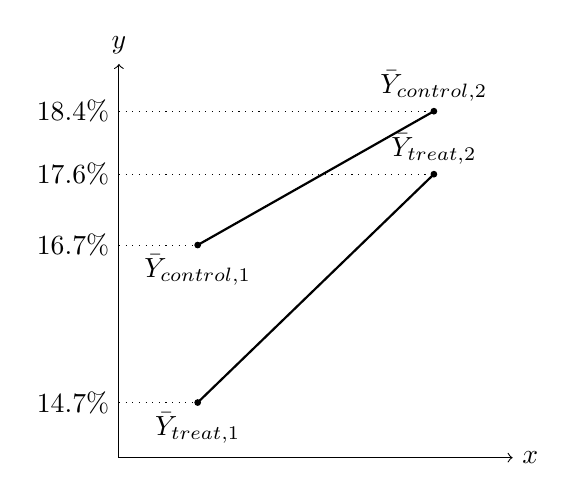
\begin{tikzpicture}
    % Draw axes
    \draw[->] (0,14) -- (5,14) node[right] {$x$};
    \draw[->] (0,14) -- (0,19) node[above] {$y$};

    % Control
    \coordinate (y_1_control) at (1, 16.7);
    \coordinate (y_2_control) at (4, 18.4);

    \filldraw (y_1_control) circle (1pt) node[below] {$\bar{Y}_{\text{control}, 1}$};
    \filldraw (y_2_control) circle (1pt) node[above] {$\bar{Y}_{\text{control}, 2}$};
    \draw[thick] (y_1_control) -- (y_2_control);


    % Treatment points
    \coordinate (y_1_treatment) at (1, 14.7);
    \coordinate (y_2_treatment) at (4, 17.6);

    \filldraw (y_1_treatment) circle (1pt) node[below] {$\bar{Y}_{\text{treat}, 1}$};
    \filldraw (y_2_treatment) circle (1pt) node[above] {$\bar{Y}_{\text{treat}, 2}$};
    \draw[thick] (y_1_treatment) -- (y_2_treatment);

    % Dotted lines
    \onslide<1>{\draw[dotted] (0,14.7) node[left] {14.7\%} -- (y_1_treatment) ;}
    \onslide<1>{\draw[dotted] (0,17.6) node[left] {17.6\%} -- (y_2_treatment) ;}
    \onslide<1>{\draw[dotted] (0,16.7) node[left] {16.7\%} -- (y_1_control) ;}
    \onslide<1>{\draw[dotted] (0,18.4) node[left] {18.4\%} -- (y_2_control) ;}

\end{tikzpicture}
\end{figure}

\textbf{Question}: How do we evaluate this treatment?
\end{column}

\begin{column}{.4\textwidth}
\end{column}
\end{columns}

\end{frame}


%%%%%%%%%%%%%%%%%%%%%%%%%%%%%%%%%%%%%%%%%%%%%%%%%%%%%%%%%%%%%%%%%%%%%%%%%%%%%%%%
\begin{frame}[t]{Differences in outcomes}

\begin{columns}
\begin{column}{.6\textwidth}

\begin{figure}
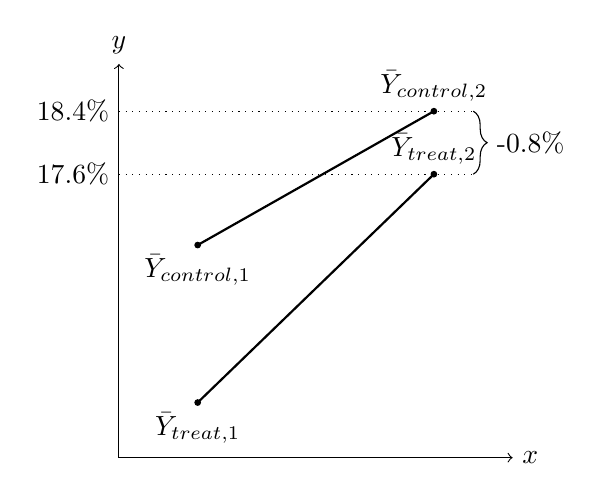
\begin{tikzpicture}
    % Draw axes
    \draw[->] (0,14) -- (5,14) node[right] {$x$};
    \draw[->] (0,14) -- (0,19) node[above] {$y$};

    % Control
    \coordinate (y_1_control) at (1, 16.7);
    \coordinate (y_2_control) at (4, 18.4);

    \filldraw (y_1_control) circle (1pt) node[below] {$\bar{Y}_{\text{control}, 1}$};
    \filldraw (y_2_control) circle (1pt) node[above] {$\bar{Y}_{\text{control}, 2}$};
    \draw[thick] (y_1_control) -- (y_2_control);


    % Treatment points
    \coordinate (y_1_treatment) at (1, 14.7);
    \coordinate (y_2_treatment) at (4, 17.6);

    \filldraw (y_1_treatment) circle (1pt) node[below] {$\bar{Y}_{\text{treat}, 1}$};
    \filldraw (y_2_treatment) circle (1pt) node[above] {$\bar{Y}_{\text{treat}, 2}$};
    \draw[thick] (y_1_treatment) -- (y_2_treatment);


    % Calligraphic brace
    \onslide<1>{\draw [decorate, decoration = {brace, amplitude=5pt}] 
        (4.5, 18.4) -- (4.5, 17.6) 
        % node[pos=0.75,left=10pt,black]{$x$}
        node [pos=0.5, right=5pt] {-0.8\%}
        ;}
    \onslide<1>{\draw[dotted] (0,17.6) node[left] {17.6\%} -- (4.5, 17.6) ;}
    \onslide<1>{\draw[dotted] (0,18.4) node[left] {18.4\%} -- (4.5, 18.4) ;}

\end{tikzpicture}

\end{figure}

\end{column}

\begin{column}{.4\textwidth}

\textbf{Method 1:} Look at the employment rate for participants after the program
    \begin{align*}
        \bar{Y}_{\text{treat}, 2} -& \bar{Y}_{\text{control}, 2} \\
        =&17.6 - 18.4 \\
        =& -0.8\%
    \end{align*}
\begin{itemize}
    \item It seems like this training program caused employment to go down
    \item Pretty unsatisfying answer, participants in the treatment group started a lower employment rate than in the control group

\end{itemize}

\end{column}
\end{columns}

\end{frame}

%%%%%%%%%%%%%%%%%%%%%%%%%%%%%%%%%%%%%%%%%%%%%%%%%%%%%%%%%%%%%%%%%%%%%%%%%%%%%%%%
\begin{frame}[t]{Differences in time}

\begin{columns}
\begin{column}{.6\textwidth}

\begin{figure}
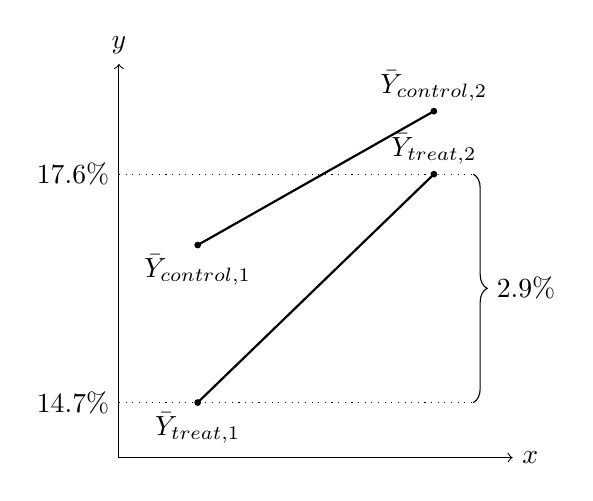
\begin{tikzpicture}
    % Draw axes
    \draw[->] (0,14) -- (5,14) node[right] {$x$};
    \draw[->] (0,14) -- (0,19) node[above] {$y$};

    % Control
    \coordinate (y_1_control) at (1, 16.7);
    \coordinate (y_2_control) at (4, 18.4);

    \filldraw (y_1_control) circle (1pt) node[below] {$\bar{Y}_{\text{control}, 1}$};
    \filldraw (y_2_control) circle (1pt) node[above] {$\bar{Y}_{\text{control}, 2}$};
    \draw[thick] (y_1_control) -- (y_2_control);


    % Treatment points
    \coordinate (y_1_treatment) at (1, 14.7);
    \coordinate (y_2_treatment) at (4, 17.6);

    \filldraw (y_1_treatment) circle (1pt) node[below] {$\bar{Y}_{\text{treat}, 1}$};
    \filldraw (y_2_treatment) circle (1pt) node[above] {$\bar{Y}_{\text{treat}, 2}$};
    \draw[thick] (y_1_treatment) -- (y_2_treatment);

    % % Dotted lines
    % \onslide<1>{\draw[dotted] (0,14.7) node[left] {14.7\%} -- (y_1_treatment) ;}
    % \onslide<1>{\draw[dotted] (0,17.6) node[left] {17.6\%} -- (y_2_treatment) ;}
    % \onslide<1>{\draw[dotted] (0,16.7) node[left] {16.7\%} -- (y_1_control) ;}
    % \onslide<1>{\draw[dotted] (0,18.4) node[left] {18.4\%} -- (y_2_control) ;}

    % % Calligraphic brace
    % \onslide<1>{\draw [decorate, decoration = {calligraphic brace, amplitude=5pt}] 
    %     (4.5, 18.4) -- (4.5, 16.7) 
    %     % node[pos=0.75,left=10pt,black]{$x$}
    %     node [pos=0.5, right=10pt] {$\Delta$}
    %     ;}

    % Calligraphic brace
    \onslide<1>{\draw [decorate, decoration = {brace, amplitude=5pt}] 
        (4.5, 17.6) -- (4.5, 14.7) 
        % node[pos=0.75,left=10pt,black]{$x$}
        node [pos=0.5, right=5pt] {2.9\%}
        ;}
    \onslide<1>{\draw[dotted] (0,17.6) node[left] {17.6\%} -- (4.5, 17.6) ;}
    \onslide<1>{\draw[dotted] (0,14.7) node[left] {14.7\%} -- (4.5, 14.7) ;}

\end{tikzpicture}
\end{figure}

\end{column}

\begin{column}{.4\textwidth}

\textbf{Method 2:} Pre-post evaluation
    \begin{align*}
        \bar{Y}_{\text{treat}, 2} - \bar{Y}_{\text{treat}, 1} =& 17.6 - 14.7 \\
        =& 2.9\%
    \end{align*}
\begin{itemize}
    \item It seems like this training program caused employment to rise
    \item Also an unsatisfying answer; employment in the control group also rose over time
    \item Maybe some external force acting on everyone (both control and treatment) that leads to higher employment rates
    \item Some of the improvement in the treatment group may be due to these external factors, not just the treatment

\end{itemize}

\end{column}
\end{columns}

\end{frame}

%%%%%%%%%%%%%%%%%%%%%%%%%%%%%%%%%%%%%%%%%%%%%%%%%%%%%%%%%%%%%%%%%%%%%%%%%%%%%%%%
\begin{frame}[t]{Differences in differences}

\begin{columns}
\begin{column}{.6\textwidth}

\begin{figure}
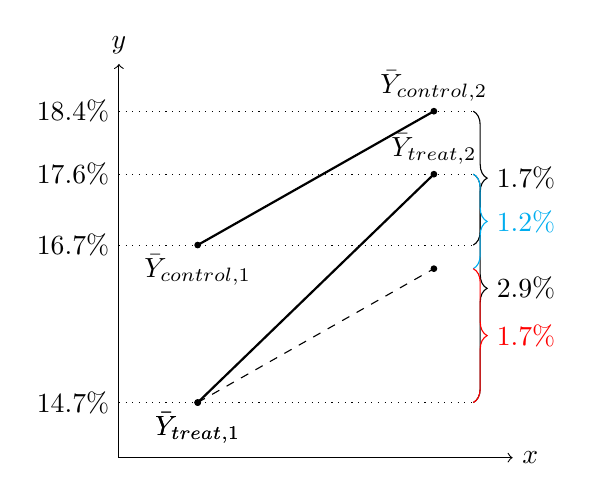
\begin{tikzpicture}
    % Draw axes
    \draw[->] (0,14) -- (5,14) node[right] {$x$};
    \draw[->] (0,14) -- (0,19) node[above] {$y$};

    % Control
    \coordinate (y_1_control) at (1, 16.7);
    \coordinate (y_2_control) at (4, 18.4);

    \filldraw (y_1_control) circle (1pt) node[below] {$\bar{Y}_{\text{control}, 1}$};
    \filldraw (y_2_control) circle (1pt) node[above] {$\bar{Y}_{\text{control}, 2}$};
    \draw[thick] (y_1_control) -- (y_2_control);


    % Treatment points
    \coordinate (y_1_treatment) at (1, 14.7);
    \coordinate (y_2_treatment) at (4, 17.6);

    \filldraw (y_1_treatment) circle (1pt) node[below] {$\bar{Y}_{\text{treat}, 1}$};
    \filldraw (y_2_treatment) circle (1pt) node[above] {$\bar{Y}_{\text{treat}, 2}$};
    \draw[thick] (y_1_treatment) -- (y_2_treatment);

    % Difference in treatment
    \onslide<1>{\draw [decorate, decoration = {brace, amplitude=5pt}] 
        (4.5, 17.6) -- (4.5, 14.7) 
        % node[pos=0.75,left=10pt,black]{$x$}
        node [pos=0.5, right=5pt] {2.9\%}
        ;}
    \onslide<1>{\draw[dotted] (0,17.6) node[left] {17.6\%} -- (4.5, 17.6) ;}
    \onslide<1>{\draw[dotted] (0,14.7) node[left] {14.7\%} -- (4.5, 14.7) ;}
    
    % Difference in control
    \onslide<2>{\draw [decorate, decoration = {brace, amplitude=5pt}] 
        (4.5, 18.4) -- (4.5, 16.7) 
        % node[pos=0.75,left=10pt,black]{$x$}
        node [pos=0.5, right=5pt] {1.7\%}
        ;}
    \onslide<2>{\draw[dotted] (0,18.4) node[left] {18.4\%} -- (4.5, 18.4) ;}
    \onslide<2>{\draw[dotted] (0,16.7) node[left] {16.7\%} -- (4.5, 16.7) ;}

    % Difference in differences
    \coordinate (y_2_treatment_null) at (4, 16.4);
    \filldraw (y_1_treatment) circle (1pt) node[below] {$\bar{Y}_{\text{treat}, 1}$};
    \onslide<3->{\filldraw (y_2_treatment_null) circle (1pt) node[below] {};}
    \onslide<3->{\draw[dashed] (y_1_treatment) -- (y_2_treatment_null);}
    \onslide<3->{\draw [cyan, decorate, decoration = {brace, amplitude=5pt}] 
        (4.5, 17.6) -- (4.5, 16.4) 
        % node[pos=0.75,left=10pt,black]{$x$}
        node [pos=0.5, right=5pt] {1.2\%}
        ;}

    \onslide<4>{\draw [decorate, red, decoration = {brace, amplitude=5pt}] 
        (4.5, 16.4) -- (4.5, 14.7)
        % node[pos=0.75,left=10pt,black]{$x$}
        node [pos=0.5, right=5pt] {1.7\%}
        ;}

\end{tikzpicture}
\end{figure}

\onslide<4>{2.9\%: Total increase in treatment group}

\onslide<4>{{\color{red}1.7\%: Increase that would have happened anyway}}
\onslide<4>{{\color{cyan}1.2\%: Treatment effect}}

\end{column}

\begin{column}{.4\textwidth}

\textbf{Method 3:} 
Compute the difference in employment for the treatment group before and after the program:
    \begin{align*}
        \bar{Y}_{\text{treat}, 2} - \bar{Y}_{\text{treat}, 1} =& 17.6 - 14.7 \\
        =& 2.9\%
    \end{align*}
\onslide<2->{Compute the difference for the control group before and after the program:
\begin{align*}
    \bar{Y}_{\text{control}, 2} - \bar{Y}_{\text{control}, 1} =& 18.4 - 16.7 \\=& 1.7\%
\end{align*}
}
\onslide<3->{Compute the differences between these differences:
\begin{equation*}
    2.9\% - 1.7\% = 1.2\%
\end{equation*}
}

\end{column}
\end{columns}

\end{frame}